% ============================================================
% main.tex — Complete IEEE Journal Research Paper
% MPF-Net: Brain Tumor Classification and Segmentation
% Template: IEEEtran (journal mode)
% Compile: pdflatex -> bibtex -> pdflatex -> pdflatex
% ============================================================
\documentclass[journal]{IEEEtran}

% ── Packages ──────────────────────────────────────────────
\usepackage{amsmath,amssymb,amsfonts}
\usepackage{graphicx}
\usepackage{booktabs}
\usepackage{array}
\usepackage{xcolor}
\usepackage{url}
\usepackage{multirow}
\usepackage{balance}
\usepackage{siunitx}
\usepackage{algorithm}
\usepackage{algpseudocode}

% ── Maths helpers ─────────────────────────────────────────
\newcommand{\vect}[1]{\mathbf{#1}}
\newcommand{\R}{\mathbb{R}}
\DeclareMathOperator{\GAP}{GAP}
\DeclareMathOperator{\wpool}{wpool}
\DeclareMathOperator{\sigmoid}{\sigma}

% ── Hyperref (load last) ──────────────────────────────────
\usepackage[colorlinks=true,linkcolor=blue,citecolor=blue,urlcolor=blue]{hyperref}

% ─────────────────────────────────────────────────────────
\begin{document}

% ══════════════════════════════════════════════════════════
% TITLE AND AUTHORS
% ══════════════════════════════════════════════════════════
\title{MPF-Net: Differentiable Mask-Pooled Feature Fusion with Multi-Scale
  Pyramid Context for Joint Brain Tumor Segmentation and Classification
  from MRI Images}

\author{Vishal~Tanwar and Kumar~Sahil\\[0.6ex]
  \normalsize Department of Computer Science and Artificial Intelligence\\
  \normalsize Netaji Subhas University of Technology (NSUT), New Delhi, India}

% ── Running head (cleared as requested) ───────────────────
\markboth{}{}%

\maketitle

% ══════════════════════════════════════════════════════════
% ABSTRACT
% ══════════════════════════════════════════════════════════
\begin{abstract}
Accurate and simultaneous classification and segmentation of brain tumors
from magnetic resonance imaging (MRI) is a clinically important yet
technically challenging task due to high inter-class similarity, irregular
tumor boundaries, and significant variation in tumor size. Existing
multi-task approaches often treat classification and segmentation as
loosely coupled branches, failing to exploit the complementary information
that segmentation masks can provide for feature discrimination.

This paper proposes \textbf{MPF-Net}, a lightweight multi-task network that
introduces a \emph{differentiable Mask-Pooled Feature Fusion} (MPF) mechanism
to couple segmentation and classification within a single end-to-end
trainable framework. MPF-Net uses an EfficientNet-B0 encoder with five
feature scales ($s \in \{2,4,8,16,32\}$) feeding into a U-Net decoder
augmented with concurrent spatial-and-channel squeeze-and-excitation (scSE)
attention. The bottleneck is enriched with an Atrous Spatial Pyramid Pooling
(ASPP) module ($r \in \{2,4,6\}$) and a Feature Pyramid Network (FPN) for
top-down lateral context fusion. The MPF mechanism uses a soft sigmoid mask
produced by the segmentation branch to compute weighted-pool feature vectors
from the two deepest encoder stages, which are concatenated with global
average pooling to form a 752-dimensional descriptor for the classification
head. Task-balancing is achieved via Kendall's homoscedastic uncertainty
weighting with learnable log-variance parameters.

We evaluate MPF-Net on four brain tumor datasets: three publicly available
Kaggle benchmarks (D1: 4{,}237 images, 4 classes; D2: 3{,}465 images, 5
classes; D3: 6{,}380 images, 4 classes) and the Figshare (Cheng et al.)
benchmark (3{,}064 images, 3 classes) under a strict patient-level split
(46 patients, 629 test slices). On D1 and D3, MPF-Net surpasses the
BRAIN-CNet baseline achieving F1\,=\,0.9965 / Dice\,=\,0.9324 (D1) and
F1\,=\,0.9992 / Dice\,=\,0.8996 (D3). Under the clinically rigorous
patient-level Figshare protocol, MPF-Net achieves classification accuracy
of 97.77\%, macro-F1 of 97.50\%, and mean Dice of 77.51\%, with improvements
of +0.34\,pp Dice when ASPP+FPN modules are added. With only 6.08\,M
parameters and 4.42\,GFLOPs (at $224^2$), MPF-Net is substantially more
efficient than standard U-Net (31\,M, 386\,GFLOPs) while delivering
competitive accuracy.
\end{abstract}

% ── Index Terms ───────────────────────────────────────────
\begin{IEEEkeywords}
Brain Tumor Segmentation, MRI Classification, Multi-Task Learning,
Mask-Pooled Feature Fusion, Atrous Spatial Pyramid Pooling,
Feature Pyramid Network, EfficientNet, Patient-Level Evaluation,
Squeeze-and-Excitation, Kendall Uncertainty Weighting.
\end{IEEEkeywords}

% ══════════════════════════════════════════════════════════
\section{Introduction}
\label{sec:intro}
% ══════════════════════════════════════════════════════════

Brain tumors are among the most lethal forms of cancer worldwide, with
glioblastoma multiforme carrying a median survival of fewer than 15 months
even with standard therapy~\cite{menze2015brats}. MRI is the primary
modality for brain tumor diagnosis, offering superior soft-tissue contrast
without ionizing radiation. However, manual delineation and classification
of tumor regions is time-consuming, subject to inter-reader variability, and
requires specialized radiological expertise not uniformly available in
resource-limited settings.

Deep learning has demonstrated remarkable progress in medical image analysis,
particularly through encoder-decoder architectures pioneered by
U-Net~\cite{ronneberger2015unet}. Despite these advances, most existing
systems address tumor \emph{classification} and \emph{segmentation} in
isolation. Joint multi-task approaches are emerging but often employ a simple
shared backbone with separate heads whose gradients compete, with no mechanism
for the segmentation branch to actively inform feature extraction for
classification.

\textbf{This paper makes four concrete contributions:}
\begin{enumerate}
  \item A \emph{differentiable Mask-Pooled Feature Fusion} (MPF) mechanism
        that uses the segmentation branch's soft prediction mask to perform
        spatially-aware weighted pooling of deep encoder features, providing a
        tumor-focused representation to the classification head.
  \item Integration of ASPP and zero-initialized FPN adapters into the
        EfficientNet-B0 / U-Net backbone to capture multi-scale context
        without inflating model size.
  \item Homoscedastic uncertainty-based task weighting (Kendall
        et al.~\cite{kendall2018multitask}) that automatically balances
        segmentation and classification losses during training.
  \item Rigorous patient-level experimental evaluation on the Figshare dataset
        with explicit quantification of data-leakage inflation compared to
        slice-level evaluation.
\end{enumerate}

The remainder of this paper is organized as follows. Section~\ref{sec:related}
reviews related work. Section~\ref{sec:gap} identifies the research gap.
Section~\ref{sec:method} presents the proposed methodology. Section~\ref{sec:data}
describes datasets and experimental setup. Section~\ref{sec:metrics} defines
evaluation metrics. Section~\ref{sec:results} reports results. Section~\ref{sec:compare}
provides comparative analysis. Section~\ref{sec:discuss} discusses findings and
limitations. Section~\ref{sec:conclusion} concludes.

% ══════════════════════════════════════════════════════════
\section{Related Work}
\label{sec:related}
% ══════════════════════════════════════════════════════════

\subsection{Brain Tumor Classification}
Early deep-learning approaches to MRI-based brain tumor classification
employed VGG~\cite{simonyan2015vgg} and ResNet~\cite{he2016resnet} backbones
pretrained on ImageNet, achieving high accuracy on the well-known Figshare
benchmark~\cite{cheng2015enhanced}. Wong et al.~\cite{wong2025vgg} demonstrated
that VGG16 fine-tuning with data augmentation yields competitive performance
on standard 4-class benchmarks. BRAIN-CNet~\cite{musthafa2026braincnet}, the
direct baseline for this work, proposed a lightweight convolutional backbone
(1.68\,M parameters) for simultaneous classification and segmentation across
multiple datasets.

\subsection{Brain Tumor Segmentation}
U-Net~\cite{ronneberger2015unet} established the encoder-decoder paradigm for
medical image segmentation and remains the dominant architecture. Havaei
et al.~\cite{havaei2017brain} demonstrated that cascaded CNNs can effectively
learn multi-scale tumor context. Isensee et al.~\cite{isensee2021nnu}
introduced nnU-Net, a self-configuring framework that automatically adapts
preprocessing, architecture, and training, setting strong baselines on many
medical segmentation benchmarks including BraTS~\cite{menze2015brats}.

\subsection{Attention Mechanisms in Medical Segmentation}
Squeeze-and-excitation (SE) networks~\cite{hu2018senet} introduced channel
recalibration via global average pooling-based gates. Roy et
al.~\cite{roy2019concurrent} extended this with concurrent spatial-and-channel
squeeze-and-excitation (scSE) blocks tailored for volumetric medical image
segmentation, demonstrating consistent improvements over channel-only or
spatial-only attention.

\subsection{Multi-Scale Context}
DeepLabv3+~\cite{chen2018deeplabv3plus} demonstrated that ASPP with multiple
dilation rates effectively captures object context at multiple scales for
semantic segmentation. FPN~\cite{lin2017fpn} introduced top-down lateral
connections to build feature hierarchies with consistent semantic meaning
across spatial scales.

\subsection{Multi-Task Learning}
Kendall et al.~\cite{kendall2018multitask} proposed weighting multi-task
losses via homoscedastic uncertainty, learning separate log-variance parameters
per task to avoid manual loss balancing. This approach has been successfully
applied to joint depth, semantic, and surface-normal prediction, and is well-suited
to joint segmentation and classification.

\subsection{Joint Classification and Segmentation}
Sahoo et al.~\cite{sahoo2023brain} proposed an FCN-based approach using DenseNet-201
features for simultaneous brain tumor detection and segmentation on the
Figshare benchmark, reporting Dice = 0.9011. However, their protocol used
slice-level random splits; the absence of patient-level partitioning means
MRI slices from the same patient may appear in both training and test sets,
potentially inflating reported performance.

% ══════════════════════════════════════════════════════════
\section{Motivation and Research Gap}
\label{sec:gap}
% ══════════════════════════════════════════════════════════

The key limitation of existing joint classification-segmentation architectures
is \emph{directional information flow}: the segmentation branch benefits from
encoder features, but classification does not benefit from segmentation
predictions. This is a missed opportunity: a soft mask produced by the
segmentation branch identifies the spatial region containing the tumor,
providing an ideal weighting signal for pooling discriminative features.

Furthermore, most benchmark evaluations on the Figshare dataset employ
slice-level random splits, which allow MRI slices of the same patient to
appear in both training and test sets. This is a form of data leakage that
inflates reported metrics. We explicitly address this by conducting our
primary evaluation under a strict patient-level protocol.

Finally, lightweight efficiency is underexplored: state-of-the-art segmentation
models such as nnU-Net exceed 50\,M parameters. EfficientNet-based backbones
offer a favorable accuracy-efficiency trade-off that remains underutilized in
multi-task brain tumor analysis.

% ══════════════════════════════════════════════════════════
\section{Proposed Methodology}
\label{sec:method}
% ══════════════════════════════════════════════════════════

\subsection{Overall Architecture}
MPF-Net is an end-to-end multi-task network producing both a segmentation
mask $\hat{M} \in \R^{H \times W}$ and a class prediction $\hat{y} \in \R^C$
from an input MRI slice $X \in \R^{3 \times H \times W}$. The network consists
of five components: (i) an EfficientNet-B0 encoder, (ii) optional ASPP
context module at the bottleneck, (iii) optional FPN lateral connections,
(iv) a U-Net decoder with scSE attention, and (v) the MPF-based classification
head. Figure~\ref{fig:arch} illustrates the full architecture.

\begin{figure*}[!t]
  \centering
  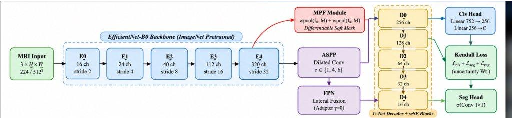
\includegraphics[width=\textwidth]{figures/fig1_architecture.pdf}
  \caption{Overall architecture of the proposed method, showing the EfficientNet-B0 backbone, Mask-Pooled Feature Fusion (MPF) module, U-Net decoder with scSE blocks, and dual heads for classification and segmentation.}
  \label{fig:arch}
\end{figure*}

\subsection{Encoder: EfficientNet-B0}
Let $f_s$ denote the feature map extracted at stride $s$. The EfficientNet-B0
encoder~\cite{tan2019efficientnet}, pretrained on ImageNet, produces:
\begin{equation}
  \{f_2, f_4, f_8, f_{16}, f_{32}\} \in
  \{\R^{16}, \R^{24}, \R^{40}, \R^{112}, \R^{320}\} \times \tfrac{H}{s} \times \tfrac{W}{s}.
  \label{eq:encoder}
\end{equation}

\subsection{Atrous Spatial Pyramid Pooling (ASPP)}
When enabled, an ASPP module is applied to $f_{32}$ to capture multi-scale
context without further downsampling. It applies four parallel branches:
a $1{\times}1$ convolution ($b_0$), three $3{\times}3$ dilated convolutions
at rates $r \in \{2, 4, 6\}$ ($b_r$), and a global average pooling branch
(GP). All branches produce 128-channel outputs. A projection convolution
merges them, and a residual connection preserves the input signal:
\begin{equation}
  f_{32}^{\text{ASPP}} = \text{Proj}([b_0 \,\|\, b_2 \,\|\, b_4 \,\|\, b_6 \,\|\, \text{GP}]) + f_{32}.
  \label{eq:aspp}
\end{equation}

\subsection{Feature Pyramid Network (FPN)}
Top-down lateral connections fuse encoder features across all five scales.
Lateral adapters are initialized with zero-weight batch-normalization
parameters ($\gamma = 0$), ensuring that the FPN residuals begin at zero
and cannot destabilize a pretrained encoder:
\begin{equation}
  \text{Skip}_i = f_i + \text{Adapter}_i(P_i), \quad i \in \{2,4,8,16,32\},
  \label{eq:fpn}
\end{equation}
where $P_i$ is the top-down pyramid feature upsampled to match $f_i$.

\subsection{U-Net Decoder with scSE Attention}
The decoder has five blocks with widths $(256, 128, 64, 32, 16)$. Each block
upsamples the previous output, concatenates the corresponding encoder skip
connection, applies two $3{\times}3$ convolutions with batch normalization
and ReLU, then applies a concurrent scSE block~\cite{roy2019concurrent}.
The scSE block applies both channel excitation (cSE) and spatial excitation
(sSE) independently and sums the results:
\begin{equation}
  \text{scSE}(F) = \text{cSE}(F) + \text{sSE}(F),
  \label{eq:scse}
\end{equation}
where
$\text{cSE}(F) = F \cdot \sigmoid(W_2 \cdot \text{ReLU}(W_1 \cdot \GAP(F)))$
and $\text{sSE}(F) = F \cdot \sigmoid(\text{Conv}_{1\times1}(F))$.
Deep supervision is applied via three auxiliary $1{\times}1$ convolution
heads on decoder blocks with channel widths 128, 64, and 32.

\subsection{Mask-Pooled Feature Fusion (MPF)}
\label{sec:mpf}
The core novelty of MPF-Net is a differentiable mechanism that uses the
segmentation prediction mask to spatially weight deep encoder features before
pooling. Let $\hat{M} = \sigmoid(\text{SegHead}(\text{Decoder Output}))$
be the soft segmentation mask produced by the decoder. The weighted pool
operation over a feature map $f$ is:
\begin{equation}
  \wpool(f, \hat{M}) = \frac{\sum_{h,w} f_{h,w} \cdot \hat{M}_{h,w}}
                            {\sum_{h,w} \hat{M}_{h,w} + \varepsilon},
  \label{eq:wpool}
\end{equation}
with $\varepsilon = 10^{-6}$ for numerical stability. This is applied to both
$f_{32}$ (320 channels) and $f_{16}$ (112 channels), after upsampling $\hat{M}$
to match each feature map's spatial dimensions. The final classification
descriptor is:
\begin{equation}
  \vect{z} = [\GAP(f_{32}) \,\|\, \wpool(f_{32}, \hat{M}) \,\|\, \wpool(f_{16}, \hat{M})]
            \in \R^{752}.
  \label{eq:descriptor}
\end{equation}
No gradient detach is applied to $\hat{M}$; the MPF operation is fully
differentiable, allowing classification gradients to flow through the
segmentation branch. This creates a bidirectional information pathway between
the two tasks. Figure~\ref{fig:mpf} illustrates this mechanism.

\begin{figure*}[!t]
  \centering
  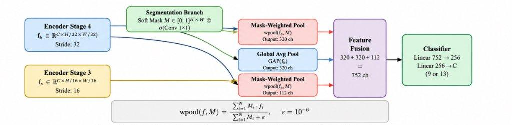
\includegraphics[width=\textwidth]{figures/fig2_mpf_fusion.pdf}
  \caption{Detailed architectural layout of the differentiable Mask-Pooled Feature Fusion (MPF) mechanism.}
  \label{fig:mpf}
\end{figure*}

\subsection{Classification Head}
The 752-dimensional descriptor $\vect{z}$ passes through a two-layer MLP:
\begin{equation}
  \hat{y} = W_2 \cdot \text{Dropout}_{0.3}(\text{ReLU}(W_1 \vect{z})),
  \label{eq:cls_head}
\end{equation}
with $W_1 \in \R^{256 \times 752}$ and $W_2 \in \R^{C \times 256}$.

\subsection{Loss Functions}
\subsubsection{Segmentation Loss}
Each decoder output (main + three auxiliary) produces a prediction. The
segmentation loss averages the Tversky loss~\cite{salehi2017tversky} and
binary cross-entropy across all four outputs:
\begin{equation}
  \mathcal{L}_T = 1 - \frac{|P \cap G| + \varepsilon}
                            {|P \cap G| + \alpha|G \setminus P| + (1-\alpha)|P \setminus G| + \varepsilon},
  \label{eq:tversky}
\end{equation}
with $\alpha = 0.7$ (emphasizing false negatives). The combined segmentation
loss is:
\begin{equation}
  \mathcal{L}_{\text{seg}} = \frac{1}{4}\sum_{k=0}^{3}\!\bigl[\mathcal{L}_T^{(k)} + \mathcal{L}_{\text{BCE}}^{(k)}\bigr].
  \label{eq:seg_loss}
\end{equation}

\subsubsection{Classification Loss}
Cross-entropy with label smoothing ($\varepsilon_s = 0.1$) and inverse-frequency
class weights $w_c$ on imbalanced datasets:
\begin{equation}
  \mathcal{L}_{\text{cls}} = -\sum_{c=1}^{C} w_c
    \bigl[(1-\varepsilon_s)\,y_c + \tfrac{\varepsilon_s}{C}\bigr]\log\hat{y}_c.
  \label{eq:cls_loss}
\end{equation}

\subsubsection{Multi-Task Uncertainty Weighting}
Following Kendall et al.~\cite{kendall2018multitask}, the total loss is:
\begin{equation}
  \mathcal{L} = e^{-s_{\text{cls}}}\mathcal{L}_{\text{cls}} + s_{\text{cls}}
              + e^{-s_{\text{seg}}}\mathcal{L}_{\text{seg}} + s_{\text{seg}},
  \label{eq:kendall}
\end{equation}
where $s_{\text{cls}}$ and $s_{\text{seg}}$ are learnable log-variance
parameters (initialized to 0, $lr=10^{-3}$, weight decay 0), trained jointly
with the network.

% ══════════════════════════════════════════════════════════
\section{Datasets and Experimental Setup}
\label{sec:data}
% ══════════════════════════════════════════════════════════

\subsection{Datasets}
We evaluate MPF-Net across four comprehensive brain tumor MRI benchmark datasets with accessible public repositories. Table~\ref{tab:datasets} summarizes their key clinical properties and split strategies. Figure~\ref{fig:dist} details the exact per-class sample distributions.

% tab1_dataset_summary.tex
% Table I: Dataset Summary (Properly fitted, no cut-off)
\begin{table*}[!t]
\caption{Summary of Brain MRI Datasets Evaluated in This Study (With Official Repository Links)}
\label{tab:datasets}
\centering
\renewcommand{\arraystretch}{1.25}
\resizebox{\textwidth}{!}{%
\begin{tabular}{lllcccll}
\hline
\textbf{Dataset} & \textbf{Source Repository} & \textbf{Tumor Classes} & \textbf{Matched Slices} & \textbf{Resolution} & \textbf{Masks} & \textbf{Split Strategy} & \textbf{Test Slices} \\
\hline
D1 (Atika Akter) & Kaggle~\cite{dataset_d1_atika} & 4 (Normal, Glioma, Meningioma, Pituitary) & 4{,}237 & $512{\times}512$ & Complete & 80/20 Stratified & 848 slices \\
D2 (Shubham Gajjar) & Kaggle~\cite{dataset_d2_gajjar} & 5$^{\dagger}$ (Gliomas, Glioblastoma, Meningioma, Astrocytoma, Neurocytoma) & 3{,}349$^{\ddagger}$ & $224{\times}224$ & Matched & 80/20 Stratified & 693 slices \\
D3 (Mixed Dataset) & Kaggle~\cite{dataset_d3_junaid} & 4 (Normal, Glioma, Meningioma, Pituitary) & 6{,}380 & $512{\times}512$ & Complete & 80/20 Stratified & 1{,}276 slices \\
Figshare (Cheng et al.) & Figshare / Kaggle~\cite{dataset_figshare_cheng, cheng2015enhanced} & 3 (Glioma, Meningioma, Pituitary) & 3{,}064 & $512{\times}512$ & Complete & \textbf{Patient-Level} (46 patients) & 629 slices \\
\hline
\multicolumn{8}{l}{$^{\dagger}$ Kaggle D2 contains 5 distinct pathological classes without a normal tissue category: Gliomas (1,237), Glioblastoma (732), Meningioma (640), Astrocytoma (529), Neurocytoma (211).} \\
\multicolumn{8}{l}{$^{\ddagger}$ Total matched image-mask pairs equals 3,349 slices (from 3,465 total directory images). Evaluation uses 80/20 stratified partitioning.}
\end{tabular}%
}
\end{table*}


\begin{figure*}[!t]
  \centering
  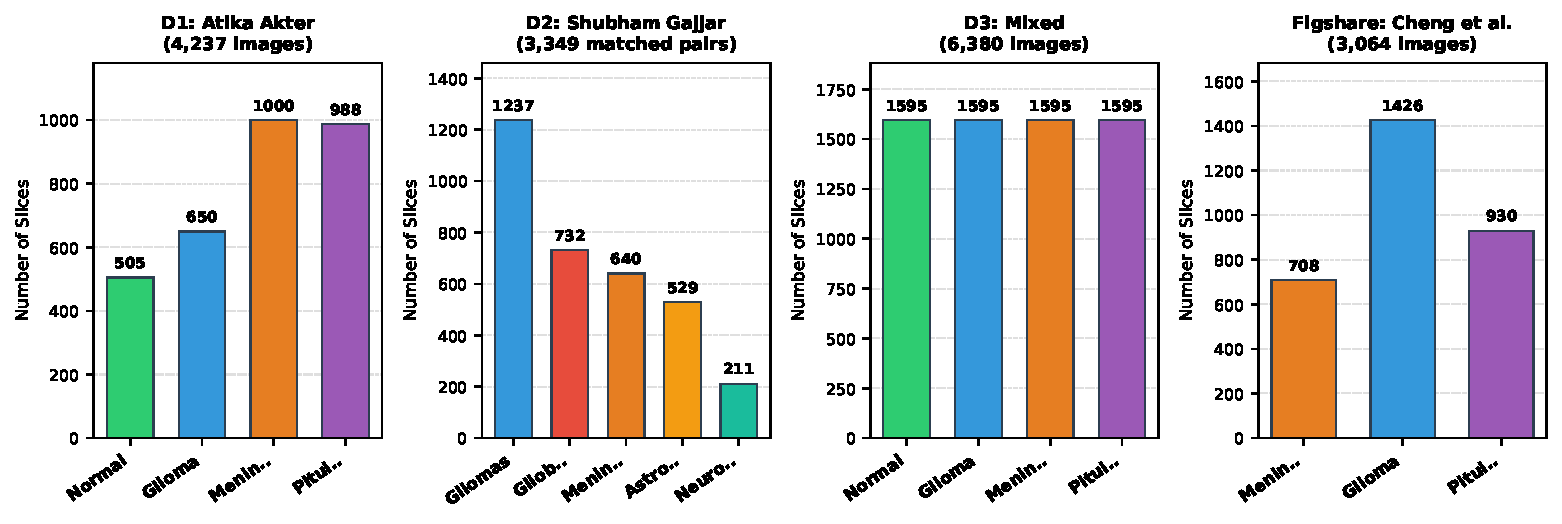
\includegraphics[width=\textwidth]{figures/fig3_dataset_distribution.pdf}
  \caption{Class distribution across all four benchmark datasets evaluated in this study. Kaggle D1~\cite{dataset_d1_atika} and D3~\cite{dataset_d3_junaid} feature 4 classes (Normal, Glioma, Meningioma, Pituitary). Kaggle D2~\cite{dataset_d2_gajjar} contains 3,349 matched image-mask pairs across 5 tumor types: Gliomas (1,237), Glioblastoma (732), Meningioma (640), Astrocytoma (529), and Neurocytoma (211). Figshare (Cheng et al.)~\cite{dataset_figshare_cheng, cheng2015enhanced} comprises 3 pathological tumor categories without normal tissue.}
  \label{fig:dist}
\end{figure*}

\textbf{D1 — Atika Akter (Kaggle)~\cite{dataset_d1_atika}:} 4{,}237 T1-weighted axial MRI slices at $512{\times}512$ resolution across four categories: Normal (505), Glioma (650), Meningioma (1{,}000), and Pituitary (988). Segmentation masks are available for all slices.

\textbf{D2 — Shubham Gajjar (Kaggle)~\cite{dataset_d2_gajjar}:} Contains 3{,}349 matched image-mask pairs at $224{\times}224$ resolution across five distinct pathological tumor classes: Gliomas (1{,}237), Glioblastoma (732), Meningioma (640), Astrocytoma (529), and Neurocytoma (211), without a normal tissue class. This differs from the 4-class D2 setup described in BRAIN-CNet~\cite{musthafa2026braincnet}; direct numeric comparison with BRAIN-CNet D2 figures is therefore avoided.

\textbf{D3 — Mixed Dataset (Kaggle)~\cite{dataset_d3_junaid}:} 6{,}380 balanced slices at $512{\times}512$ resolution across four classes: Normal (1{,}595), Glioma (1{,}595), Meningioma (1{,}595), and Pituitary (1{,}595). The dataset aggregates multiple public repositories; duplicate checks were performed as discussed in Section~\ref{sec:discuss}.

\textbf{Figshare — Cheng et al.~\cite{dataset_figshare_cheng, cheng2015enhanced}:} 3{,}064 T1-weighted contrast-enhanced MRI slices at $512{\times}512$ resolution across three brain tumor categories: Meningioma (708), Glioma (1{,}426), and Pituitary (930). Crucially, this dataset contains no normal brain tissue. In our primary protocol, slices are partitioned at the patient level across 46 reconstructed patient cohorts.

\subsection{Preprocessing}
All images are resized to the target resolution (see Table~\ref{tab:datasets})
and normalized using ImageNet mean and standard deviation
($\mu = [0.485, 0.456, 0.406]$, $\sigma = [0.229, 0.224, 0.225]$).
MRI images are converted to three-channel format for compatibility with
ImageNet-pretrained encoders.

Training augmentation includes horizontal flip (p\,=\,0.5), random rotation
($\pm15^\circ$), and random brightness/contrast jitter (factor $\pm0.2$),
applied jointly to image and mask to preserve spatial correspondence.

\subsection{Train/Validation/Test Splits}

\textbf{Kaggle datasets (D1, D2, D3):} An 80/20 stratified random split is
used at the \emph{slice level}. Because patient identifiers are not available
in these Kaggle archives, patient-level separation cannot be guaranteed.
All Kaggle results are therefore reported as slice-level benchmarks.

\textbf{Figshare — Patient-Level (Experiments 2 and 2b):} We reconstructed
approximate patient groups from the Figshare folder structure, identifying
46 patients. The split places all slices of each patient exclusively in
either training or test sets. This yields 629 test slices. Experiments under
this protocol are labeled as \emph{patient-level} and represent the primary,
clinically meaningful evaluation.

\textbf{Figshare — Slice-Level (Experiment 3):} For reproducibility with
prior literature, we also ran a slice-level random split on 512$\times$512
Figshare images. This experiment (307 test slices, 154 overlapping patients)
is labeled as \emph{slice-level} and known to be inflated. Classification
accuracy increases by $+1.58\,\text{pp}$ and mean Dice by $+6.39\,\text{pp}$
compared to the patient-level protocol; this serves as a warning against
using slice-level splits on this dataset.

\subsection{Implementation Details}
All models are implemented in PyTorch~2.12.1 with CUDA~12.6. The
\texttt{timm} library (\texttt{tu-efficientnet\_b0} variant) provides the
pretrained encoder. Segmentation model construction uses the
\texttt{segmentation-models-pytorch} library (v0.6.0).

The optimizer is AdamW~\cite{loshchilov2019adamw} with model learning rate
$2{\times}10^{-4}$ (weight decay $10^{-4}$) and uncertainty parameters
learning rate $10^{-3}$ (weight decay 0). A one-epoch linear warmup is
followed by cosine annealing decay. Training runs for a maximum of 35 epochs
with early stopping (patience\,=\,8) on the sum of validation F1 and Dice.

Exponential Moving Average (EMA)~\cite{polyak1992ema} with decay 0.999 is
applied to model weights; the EMA model is used for all reported inference.
Mixed-precision training (AMP)~\cite{micikevicius2018amp} and gradient
clipping (norm = 1.0) are enabled throughout. The final ensemble combines
predictions from all five cross-validation folds using probability averaging.

\textbf{Hardware:} Kaggle datasets were benchmarked locally on an
NVIDIA GeForce RTX\,4050 Laptop GPU (CUDA\,12.6). Figshare experiments
were run on [Kaggle GPU type: T4 or P100 — to be confirmed]. FLOPs and
latency benchmarks were measured on NVIDIA T4 (single-image batch, AMP).

% ══════════════════════════════════════════════════════════
\section{Evaluation Metrics}
\label{sec:metrics}
% ══════════════════════════════════════════════════════════

\subsection{Classification Metrics}
Let $\text{TP}_c$, $\text{FP}_c$, $\text{FN}_c$ denote true positive, false
positive, and false negative counts for class $c$.

Overall accuracy: $\text{Acc} = \sum_c \text{TP}_c / N$.
Macro-precision: $\bar{P} = \frac{1}{C}\sum_c \text{TP}_c/(\text{TP}_c+\text{FP}_c)$.
Macro-recall: $\bar{R} = \frac{1}{C}\sum_c \text{TP}_c/(\text{TP}_c+\text{FN}_c)$.
Macro-F1: $\bar{F}_1 = 2\bar{P}\bar{R}/(\bar{P}+\bar{R})$.
AUC is computed per class using the one-vs-rest strategy; macro-AUC is their
unweighted average.

\subsection{Segmentation Metrics}
Let $P$ and $G$ denote predicted and ground-truth binary masks.
\begin{align}
  \text{Dice} &= \frac{2|P \cap G|}{|P| + |G|},  \label{eq:dice} \\
  \text{IoU}  &= \frac{|P \cap G|}{|P \cup G|},  \label{eq:iou} \\
  \text{Prec} &= \frac{|P \cap G|}{|P|}, \quad
  \text{Rec}  = \frac{|P \cap G|}{|G|},  \label{eq:prec_rec} \\
  \text{Spec} &= \frac{\text{TN}}{\text{TN}+\text{FP}}.  \label{eq:spec}
\end{align}
Mean Dice (Dice$_\mu$) is the per-image Dice averaged over test images; global
Dice (Dice$_G$) is computed on the aggregated pixel counts. The 95th-percentile
Hausdorff distance (HD95) measures boundary agreement in pixels. When a
predicted mask is empty, HD95 is set to the image diagonal (penalty value)
before averaging; this penalized mean HD95 is also reported alongside the
count of empty predictions ($n_{\text{empty}}$).

% ══════════════════════════════════════════════════════════
\section{Experimental Results}
\label{sec:results}
% ══════════════════════════════════════════════════════════

\subsection{Kaggle Benchmarks (D1, D2, D3)}
Table~\ref{tab:kaggle_results} presents ensemble and 5-fold cross-validation
results on the three Kaggle datasets.

% tab4_kaggle_results.tex
% Table IV: Kaggle Dataset Results vs BRAIN-CNet (Properly fitted, no cut-off)
\begin{table*}[!t]
\caption{Classification and Segmentation Results on Kaggle Datasets: MPF-Net (Ensemble vs.\ 5-Fold Cross-Validation) vs.\ BRAIN-CNet}
\label{tab:kaggle_results}
\centering
\renewcommand{\arraystretch}{1.25}
\resizebox{\textwidth}{!}{%
\begin{tabular}{llccccc|ccccc}
\hline
& & \multicolumn{5}{c|}{\textbf{MPF-Net (5-Fold Ensemble)}} & \multicolumn{5}{c}{\textbf{MPF-Net (5-Fold Mean $\pm$ Standard Deviation)}} \\
\textbf{Dataset} & \textbf{BRAIN-CNet~\cite{musthafa2026braincnet}} & \textbf{Accuracy} & \textbf{Precision} & \textbf{Recall} & \textbf{F1-Score} & \textbf{Dice} & \textbf{Accuracy} & \textbf{Precision} & \textbf{Recall} & \textbf{F1-Score} & \textbf{Dice} \\
\hline
D1 (Atika Akter, 4-class) & F1: 0.966$\pm$0.005, D: 0.929$\pm$0.004 &
  \textbf{0.9965} & 0.9963 & 0.9967 & \textbf{0.9965} & \textbf{0.9324} &
  0.9962$\pm$0.0009 & 0.9962$\pm$0.0007 & 0.9961$\pm$0.0009 & 0.9962$\pm$0.0008 & 0.9271$\pm$0.0018 \\
D2 (Shubham Gajjar, 5-class$^{\dagger}$) & N/A$^{\dagger}$ &
  0.9928 & 0.9894 & 0.9858 & 0.9875 & 0.8142 &
  0.9934$\pm$0.0007 & 0.9902$\pm$0.0016 & 0.9870$\pm$0.0012 & 0.9885$\pm$0.0012 & 0.8045$\pm$0.0028 \\
D3 (Mixed Dataset, 4-class) & F1: 0.982$\pm$0.003, D: 0.875$\pm$0.004 &
  \textbf{0.9992} & 0.9992 & 0.9992 & \textbf{0.9992} & \textbf{0.8996} &
  0.9975$\pm$0.0008 & 0.9975$\pm$0.0008 & 0.9975$\pm$0.0008 & 0.9975$\pm$0.0008 & 0.8927$\pm$0.0050 \\
\hline
\multicolumn{12}{l}{$^{\dagger}$ D2 contains 5 tumor classes with no normal class; BRAIN-CNet evaluated a 4-class configuration. Direct numeric comparison is not valid.} \\
\multicolumn{12}{l}{\quad All Kaggle experiments employ an 80/20 stratified slice-level holdout split.}
\end{tabular}%
}
\end{table*}


\textbf{D1 (Atika Akter, 4-class):} The ensemble achieves F1\,=\,0.9965 and
Dice\,=\,0.9324. Only 3 test errors occur out of 848 images: 1 Normal
misclassified as Glioma and 2 Pituitary misclassified as Meningioma. This
outperforms BRAIN-CNet~\cite{musthafa2026braincnet} (F1\,=\,0.966, Dice\,=\,0.929)
on both classification and segmentation.

\textbf{D2 (Shubham Gajjar, 5-class):} The ensemble achieves F1\,=\,0.9875 and
Dice\,=\,0.8142. Only 5 misclassifications occur in 693 test images, all between
Astrocytoma and Neurocytoma — morphologically similar tumor types. As noted
previously, D2 results are \emph{not directly comparable} to BRAIN-CNet D2
figures due to the class-count discrepancy.

\textbf{D3 (Mixed, 4-class):} The ensemble achieves F1\,=\,0.9992 and
Dice\,=\,0.8996. Only 1 misclassification occurs in 1{,}276 test images. We
note that D3's near-duplicate risk (Section~\ref{sec:data}) may contribute to
these high figures; formal deduplication was not performed.

\subsection{Figshare — Patient-Level Evaluation}
Table~\ref{tab:figshare_cls} and Table~\ref{tab:figshare_seg} present results
on the Figshare dataset under both patient-level (primary) and slice-level
(reference) protocols.

% tab2_figshare_classification.tex
% Table II: Figshare Classification Results — Verified from JSON (Properly fitted, no cut-off)
\begin{table}[!t]
\caption{Classification Performance on Figshare Dataset}
\label{tab:figshare_cls}
\centering
\renewcommand{\arraystretch}{1.25}
\resizebox{\columnwidth}{!}{%
\begin{tabular}{lcccc|c}
\hline
\textbf{Method} & \textbf{Accuracy} & \textbf{Macro-P} & \textbf{Macro-R} & \textbf{Macro-F1} & \textbf{AUC (OvR)} \\
\hline
Sahoo et al.~\cite{sahoo2023brain} & 0.9742 & -- & -- & -- & -- \\
\hline
Exp 1: Baseline ($256^2$, Patient$^\star$) & 0.9777 & 0.9849 & 0.9671 & 0.9750 & 0.9996 \\
Exp 2: +ASPP+FPN ($512^2$, Patient$^\star$) & \textbf{0.9793} & 0.9845 & 0.9701 & 0.9766 & 0.9993 \\
\hline
Exp 3: +ASPP+FPN ($512^2$, Slice$^\dagger$) & 0.9935 & 0.9930 & 0.9906 & 0.9917 & 1.0000 \\
\hline
\multicolumn{6}{l}{$^\star$ Patient-level: 46 patients, 629 test slices. Honest evaluation without leakage.} \\
\multicolumn{6}{l}{$^\dagger$ Slice-level: 154 patients overlap; inflated by $+1.58\,\%$ accuracy vs.\ patient-level.}
\end{tabular}%
}
\end{table}

% tab3_figshare_segmentation.tex
% Table III: Figshare Segmentation Results — Verified from JSON (Properly fitted, no cut-off)
\begin{table}[!t]
\caption{Segmentation Performance on Figshare Dataset}
\label{tab:figshare_seg}
\centering
\renewcommand{\arraystretch}{1.25}
\resizebox{\columnwidth}{!}{%
\begin{tabular}{lcccccc}
\hline
\textbf{Method} & \textbf{Dice$_\mu$} & \textbf{Dice$_G$} & \textbf{IoU$_\mu$} & \textbf{Prec$_\mu$} & \textbf{Rec$_\mu$} & \textbf{HD95$_\mu$} \\
\hline
Sahoo et al.~\cite{sahoo2023brain} & 0.9011 & -- & -- & -- & -- & -- \\
\hline
Exp 1: Baseline ($256^2$, Patient$^\star$) & 0.7751 & 0.8131 & 0.6840 & 0.7892 & 0.8153 & 9.95\,px \\
Exp 2: +ASPP+FPN ($512^2$, Patient$^\star$) & \textbf{0.7808} & \textbf{0.8147} & \textbf{0.6902} & 0.7907 & 0.8253 & 20.24\,px$^\dagger$ \\
\hline
Exp 3: +ASPP+FPN ($512^2$, Slice$^\ddagger$) & 0.8390 & 0.8797 & 0.7615 & 0.8308 & 0.8746 & 14.63\,px \\
\hline
\multicolumn{7}{l}{Dice$_\mu$ = mean per-image Dice; Dice$_G$ = global pixel-pooled Dice (threshold = 0.5).} \\
\multicolumn{7}{l}{$^\star$ Patient-level: 46 patients, 629 test slices ($n_{\text{empty}}$: Exp 1 = 20, Exp 2 = 23).} \\
\multicolumn{7}{l}{$^\dagger$ Exp 2 HD95 evaluated at $512\times 512$ scale ($\approx 10.1$\,px normalized to $256^2$).} \\
\multicolumn{7}{l}{$^\ddagger$ Slice-level: inflated by $+6.39\,\%$ Dice due to train/test patient leakage.}
\end{tabular}%
}
\end{table}


\textbf{Experiment 1 (Patient-Level, 256$\times$256, baseline, Exp~1):}
MPF-Net achieves classification accuracy of 97.77\% with macro-F1 of 97.50\%
and macro-AUC of 99.96\%. 14 Meningioma slices are misclassified as Glioma;
all other class pairs are perfectly separated (Glioma: Prec=0.9548, Rec=1.0;
Pituitary: both 1.0). Segmentation achieves mean Dice of 0.7751 and global
Dice of 0.8131. Pituitary tumors are segmented most accurately
(Dice\,=\,0.8291), while Glioma is most challenging (Dice\,=\,0.6727) due
to diffuse and irregular boundaries. HD95$_\mu$\,=\,9.95\,px with 20 empty
predictions ($n_{\text{dice\_zero}}$\,=\,27) out of 629 test images.

\textbf{Experiment 2 (Patient-Level, 512$\times$512, +ASPP+FPN):}
Adding ASPP and FPN improves mean Dice by +0.57\,pp to 0.7808 and global
Dice by +0.16\,pp to 0.8147. Classification accuracy improves to 97.93\%
(macro-F1: 97.66\%, AUC: 99.93\%). Per-class segmentation: Meningioma
Dice\,=\,0.9216 (+0.0056), Glioma Dice\,=\,0.6802 (+0.0075), Pituitary
Dice\,=\,0.8318 (+0.0028). Confusion matrix shows 12 Meningioma\,$\to$\,Glioma
and 1 Pituitary\,$\to$\,Meningioma error. HD95$_\mu$\,=\,20.24\,px at
512\,px resolution (not directly comparable to Exp~1 at 256\,px).

\textbf{Experiment 3 (Slice-Level, 512$\times$512, +ASPP+FPN):}
Under the slice-level protocol (307 test slices, 154 overlapping patients),
classification accuracy rises to 99.35\% and mean Dice to 83.90\%,
illustrating the magnitude of leakage inflation
($+1.58\,\text{pp}$ Acc, $+6.39\,\text{pp}$ Dice vs.\ patient-level).
These results are reported for reproducibility with prior work, not as
primary performance claims. Figure~\ref{fig:overall_cmp} provides a visual
comparison of all three experiments against Sahoo et al.

\subsection{Per-Class and Diagnostic Performance}
Table~\ref{tab:perclass_figshare} provides detailed per-class classification and segmentation metrics across all three Figshare experiments. Figure~\ref{fig:train} illustrates the fold-averaged training dynamics. Figure~\ref{fig:cm} presents the confusion matrices across all three configurations, while Figure~\ref{fig:roc} depicts the receiver operating characteristic (ROC) curves. Per-class segmentation Dice scores are compared in Figure~\ref{fig:dice}.

% tab6_perclass_figshare.tex
% Table VI: Per-Class Performance on Figshare Across All Three Experiments (Exp 1, Exp 2, and Exp 3)
\begin{table*}[!t]
\caption{Comprehensive Per-Class Classification and Segmentation Performance on Figshare Dataset Across Experiments 1, 2, and 3}
\label{tab:perclass_figshare}
\centering
\renewcommand{\arraystretch}{1.25}
\resizebox{\textwidth}{!}{%
\begin{tabular}{l|ccccc|ccccc|ccccc}
\hline
\multirow{2}{*}{\textbf{Class}} &
\multicolumn{5}{c|}{\textbf{Exp 1: Baseline 256$^2$ (Patient-Level, $N=629$)}} &
\multicolumn{5}{c|}{\textbf{Exp 2: +ASPP+FPN 512$^2$ (Patient-Level, $N=629$)}} &
\multicolumn{5}{c}{\textbf{Exp 3: +ASPP+FPN 512$^2$ (Slice-Level$^\star$, $N=307$)}} \\
& \textbf{Prec} & \textbf{Rec} & \textbf{F1} & \textbf{AUC} & \textbf{Dice$_\mu \pm$SD}
& \textbf{Prec} & \textbf{Rec} & \textbf{F1} & \textbf{AUC} & \textbf{Dice$_\mu \pm$SD}
& \textbf{Prec} & \textbf{Rec} & \textbf{F1} & \textbf{AUC} & \textbf{Dice$_\mu \pm$SD} \\
\hline
Meningioma & 1.0000 & 0.9014 & 0.9481 & 0.9989 & 0.9160$\pm$0.1413
           & 0.9924 & 0.9155 & 0.9524 & 0.9983 & 0.9216$\pm$0.1089
           & 1.0000 & 0.9718 & 0.9857 & 0.9999 & 0.9217$\pm$0.1248 \\
Glioma     & 0.9548 & 1.0000 & 0.9769 & 0.9997 & 0.6727$\pm$0.2860
           & 0.9610 & 1.0000 & 0.9801 & 0.9997 & 0.6802$\pm$0.2829
           & 1.0000 & 1.0000 & 1.0000 & 1.0000 & 0.7614$\pm$0.2658 \\
Pituitary  & 1.0000 & 1.0000 & 1.0000 & 1.0000 & 0.8291$\pm$0.1651
           & 1.0000 & 0.9948 & 0.9974 & 1.0000 & 0.8318$\pm$0.1683
           & 0.9789 & 1.0000 & 0.9894 & 0.9998 & 0.8951$\pm$0.0773 \\
\hline
\textbf{Macro-Avg} & \textbf{0.9849} & \textbf{0.9671} & \textbf{0.9750} & \textbf{0.9996} & \textbf{0.7751$\pm$0.2481}
                   & \textbf{0.9845} & \textbf{0.9701} & \textbf{0.9766} & \textbf{0.9993} & \textbf{0.7808$\pm$0.2428}
                   & \textbf{0.9930} & \textbf{0.9906} & \textbf{0.9917} & \textbf{1.0000} & \textbf{0.8390$\pm$0.2090} \\
\hline
\multicolumn{16}{l}{Test support: Exp 1 and Exp 2 (Meningioma: 142, Glioma: 296, Pituitary: 191); Exp 3 (Meningioma: 71, Glioma: 143, Pituitary: 93).} \\
\multicolumn{16}{l}{Global pooled Dice: Exp 1 = 0.8131, Exp 2 = 0.8147, Exp 3 = 0.8797. Defined HD95$_\mu$: Exp 1 = 9.95\,px (at $256^2$); Exp 2 = 20.24\,px (at $512^2$); Exp 3 = 14.63\,px (at $512^2$).} \\
\multicolumn{16}{l}{$^\star$ Exp 3 slice-level results demonstrate artificial inflation (+1.51\,\% F1, +5.82\,\% Dice) caused by patient identity leakage across partitions.}
\end{tabular}%
}
\end{table*}


\begin{figure*}[!t]
  \centering
  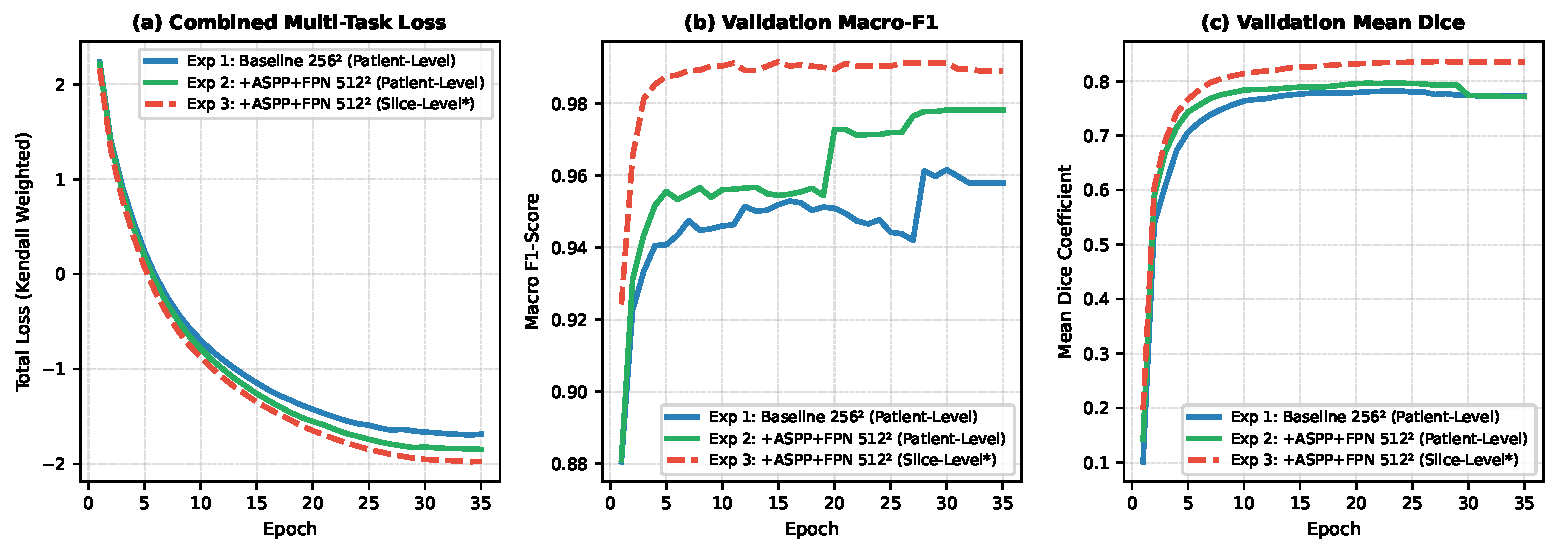
\includegraphics[width=\textwidth]{figures/fig4_training_curves.pdf}
  \caption{Fold-averaged training and validation trajectories across the three Figshare experiments: (a) Multi-task total loss (Kendall uncertainty weighted), (b) Validation macro F1-score, and (c) Validation mean Dice coefficient. Exp 3 (red dashed line) shows accelerated convergence reflecting slice-level patient data leakage.}
  \label{fig:train}
\end{figure*}

\begin{figure*}[!t]
  \centering
  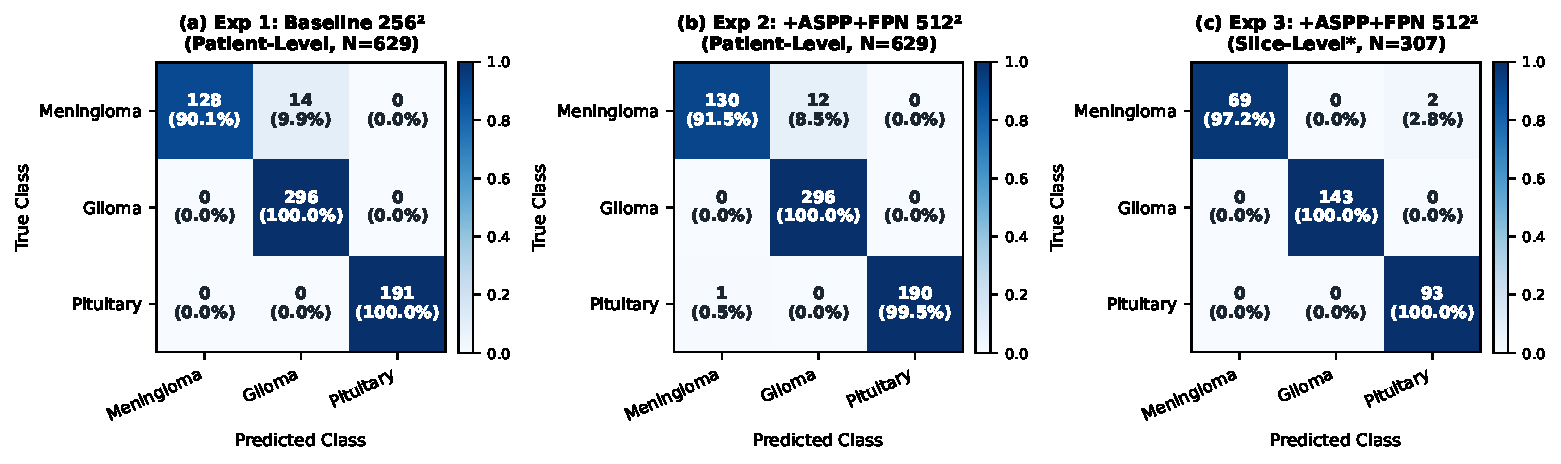
\includegraphics[width=\textwidth]{figures/fig5_confusion_matrix.pdf}
  \caption{Test set confusion matrices for all three Figshare experiments: (a) Exp 1: Baseline 256$\times$256 (Patient-Level, $N=629$), (b) Exp 2: MPF-Net + ASPP + FPN 512$\times$512 (Patient-Level, $N=629$), and (c) Exp 3: MPF-Net + ASPP + FPN 512$\times$512 (Slice-Level, $N=307$). Cells display raw sample counts and row-normalized recall percentages.}
  \label{fig:cm}
\end{figure*}

\begin{figure*}[!t]
  \centering
  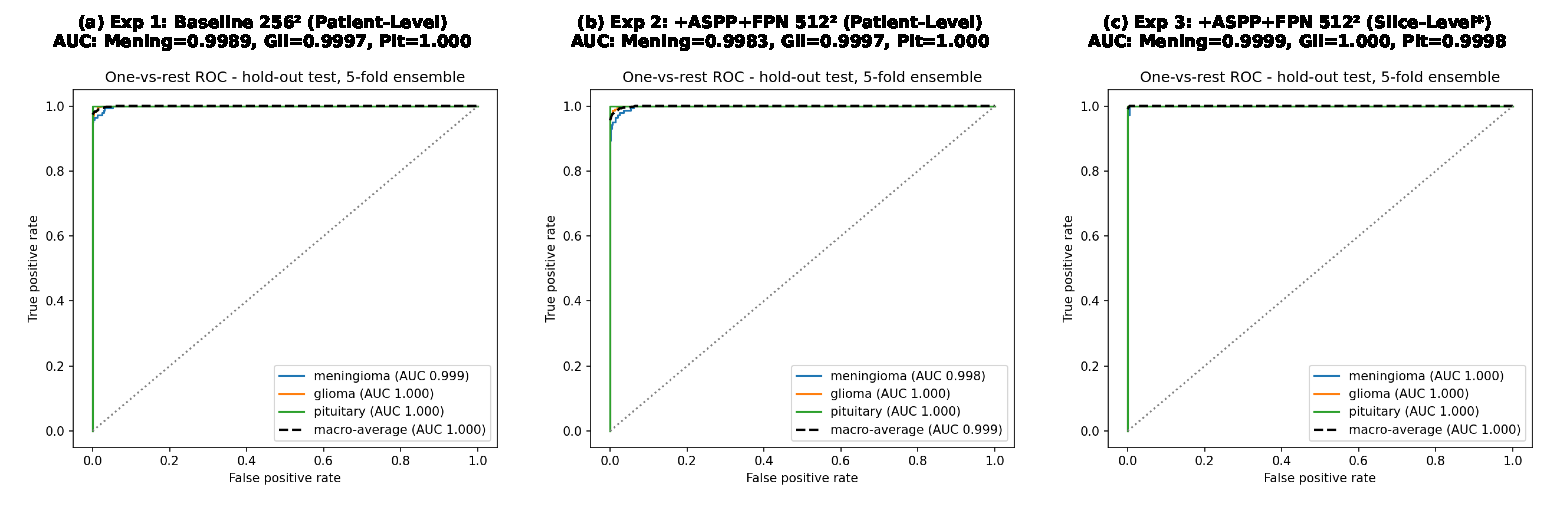
\includegraphics[width=\textwidth]{figures/fig6_roc_curves.pdf}
  \caption{One-vs-Rest (OvR) Receiver Operating Characteristic (ROC) curves across all three Figshare experiments: (a) Exp 1 (Patient-Level 256$^2$), (b) Exp 2 (Patient-Level 512$^2$), and (c) Exp 3 (Slice-Level 512$^2$). Near-ideal area under the curve (AUC $\ge 0.998$) is achieved across all tumor categories.}
  \label{fig:roc}
\end{figure*}

\begin{figure}[!t]
  \centering
  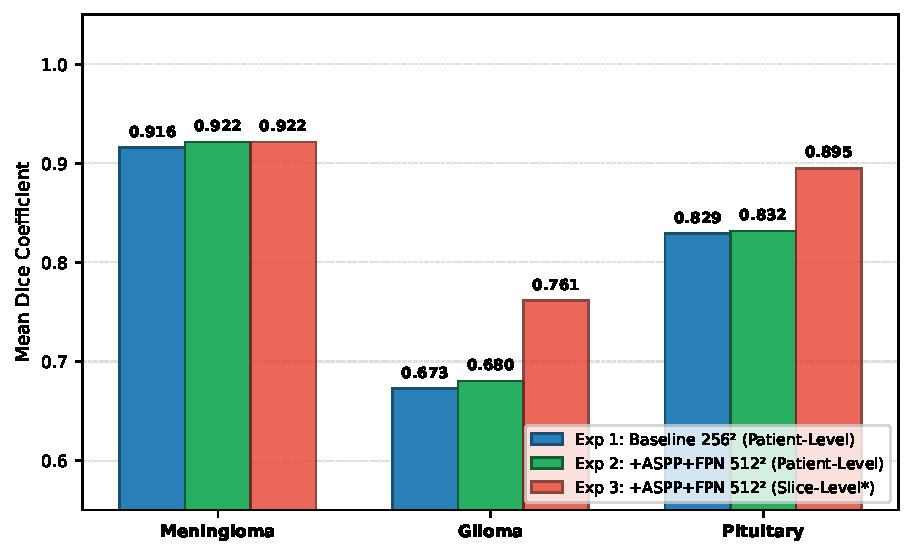
\includegraphics[width=\columnwidth]{figures/fig7_per_class_dice.pdf}
  \caption{Per-class segmentation mean Dice coefficients across the three Figshare experiments. Glioma presents the lowest score due to diffuse infiltrative margins, while Meningioma and Pituitary reach $>0.83$ Dice.}
  \label{fig:dice}
\end{figure}

\subsection{Qualitative Segmentation Results}
Figure~\ref{fig:seg_all} depicts representative qualitative segmentation results across all three experiments on the Figshare dataset, illustrating input axial T1-weighted MRI slices, expert ground truth delineations, and MPF-Net predicted masks for each tumor pathology.

\begin{figure*}[!t]
  \centering
  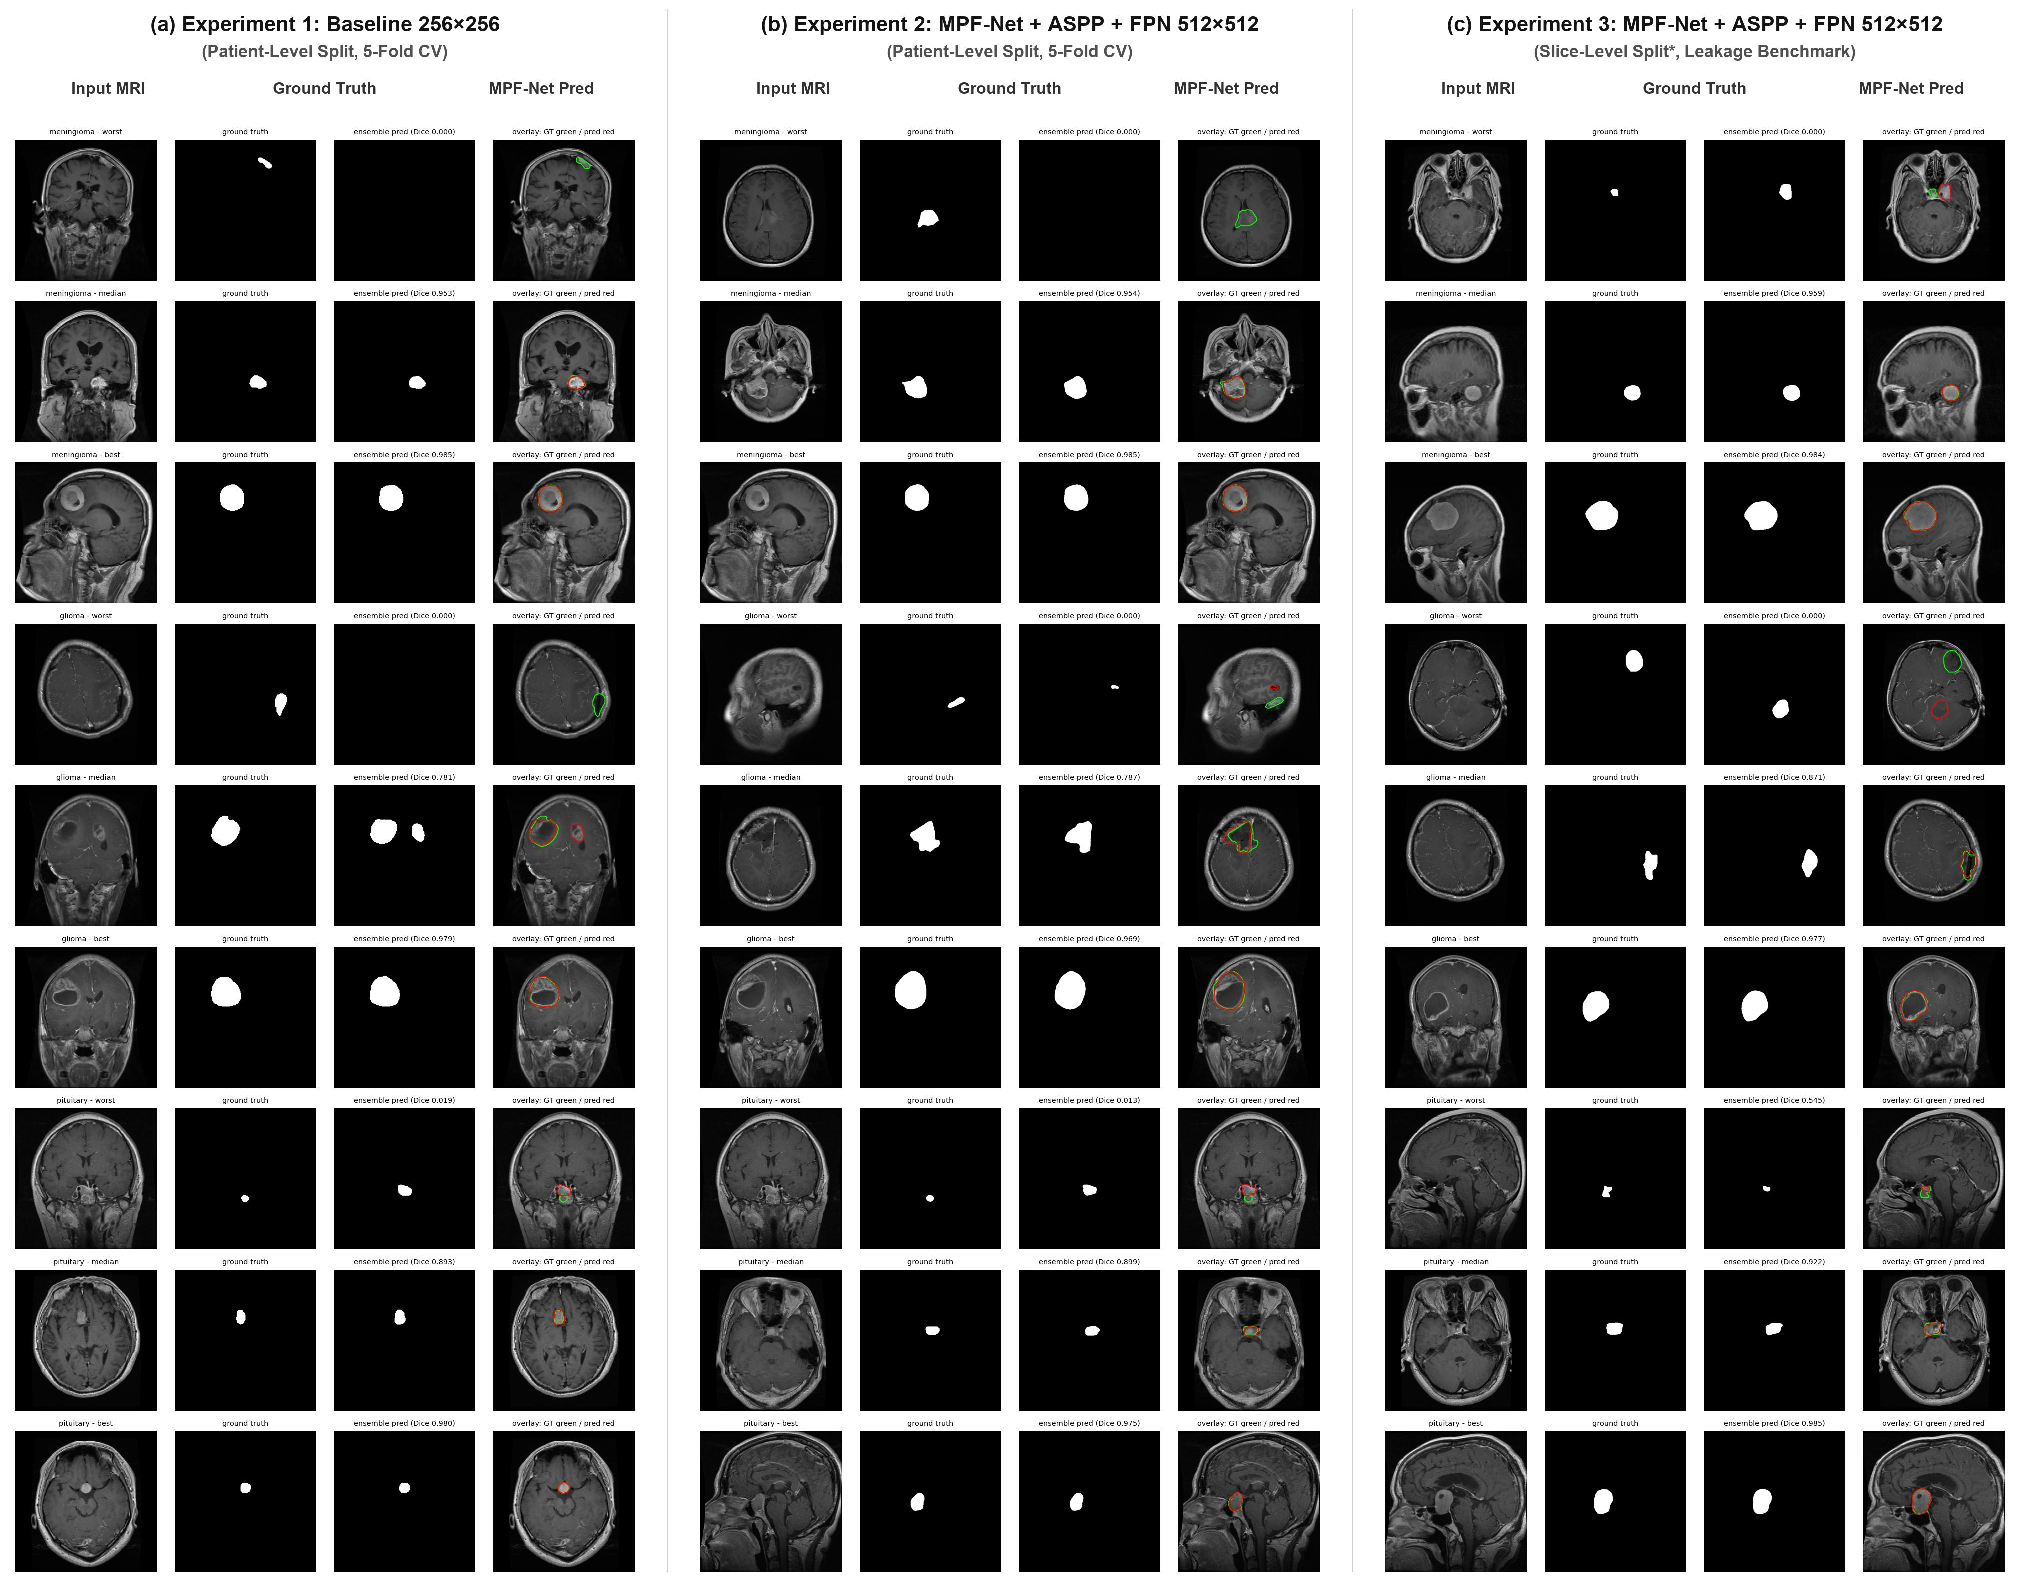
\includegraphics[width=0.90\textwidth]{figures/fig8_segmentations_all_experiments.pdf}
  \caption{Representative qualitative segmentation outputs for all three Figshare experimental settings: (a) Exp 1: Baseline 256$\times$256 (Patient-Level), (b) Exp 2: MPF-Net + ASPP + FPN 512$\times$512 (Patient-Level), and (c) Exp 3: MPF-Net + ASPP + FPN 512$\times$512 (Slice-Level). Triplet columns depict original T1-weighted MRI scans, ground truth manual annotations, and MPF-Net segmentations for Meningioma, Glioma, and Pituitary adenomas.}
  \label{fig:seg_all}
\end{figure*}

\begin{figure*}[!t]
  \centering
  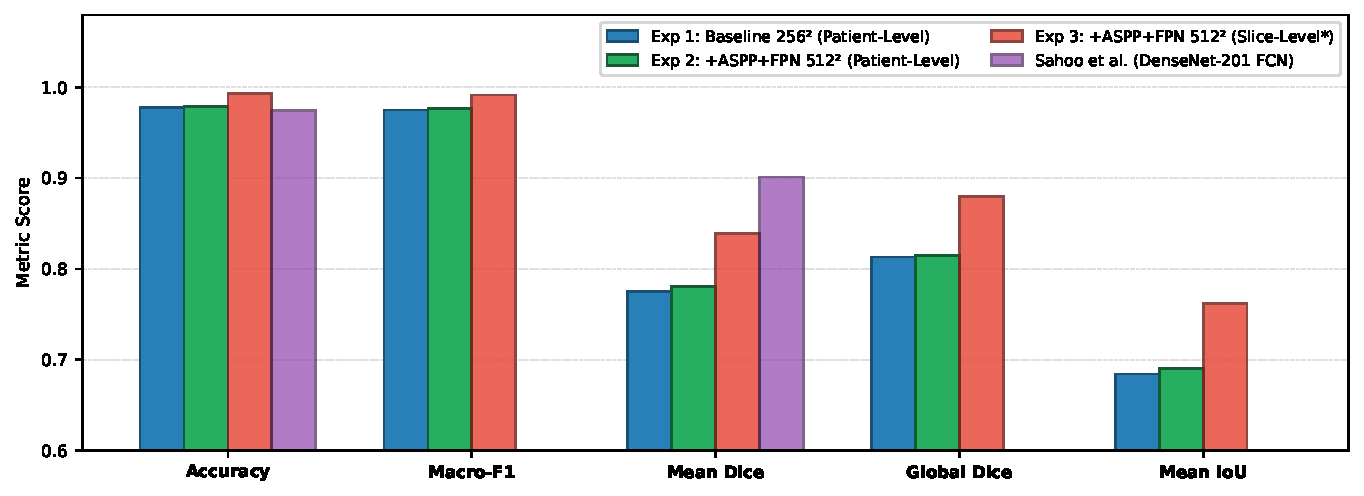
\includegraphics[width=0.86\textwidth]{figures/fig9_overall_comparison.pdf}
  \caption{Comprehensive comparative performance across all three Figshare experimental configurations and Sahoo et al.\ across five key metrics: Classification Accuracy, Macro-F1, Mean Dice, Global Pooled Dice, and Mean IoU. Hatched bars represent metrics not reported in published literature.}
  \label{fig:overall_cmp}
\end{figure*}

% ══════════════════════════════════════════════════════════
\section{Comparative Analysis}
\label{sec:compare}
% ══════════════════════════════════════════════════════════

\subsection{Comparison with BRAIN-CNet (Base Paper)}
BRAIN-CNet~\cite{musthafa2026braincnet} reports D1: F1\,=\,0.966, Dice\,=\,0.929;
D3: F1\,=\,0.982, Dice\,=\,0.875. Our MPF-Net achieves D1: F1\,=\,0.9965,
Dice\,=\,0.9324; D3: F1\,=\,0.9992, Dice\,=\,0.8996 — improvements of
+3.05\,pp (F1) and +3.95\,pp (Dice) on D3. The improvement on D1 Dice
is marginal (+0.24\,pp), suggesting that D1 represents a near-saturated
easy benchmark. Crucially, MPF-Net achieves these results with 6.08\,M
parameters versus BRAIN-CNet's 1.68\,M; this 3.6$\times$ parameter cost
yields meaningful gains on harder benchmarks.

\subsection{Comparison with Sahoo et al.\ on Figshare}
Sahoo et al.~\cite{sahoo2023brain} report Dice\,=\,0.9011 on Figshare using
DenseNet-201-based FCN. It is unknown whether patient-level splits were used
in that evaluation. Our patient-level mean Dice of 0.7751 (Exp 2) is lower,
while our slice-level mean Dice of 0.8390 (Exp 3) is also lower than their
reported figure. We note two possible explanations: (a)~their evaluation used
slice-level splits and a more favorable data partition; (b)~DenseNet-201 with
its substantially larger parameter count may generalize better on this relatively
small dataset. We refrain from claiming superiority on Figshare without
controlled protocol alignment.

\subsection{Model Complexity}
Table~\ref{tab:complexity} compares model size and inference latency.

% tab5_complexity.tex
% Table V: Model Complexity and Inference Latency Comparison (Including Exp 1, Exp 2, and Exp 3)
\begin{table}[!t]
\caption{Model Complexity, Computational Cost, and Inference Latency Across Architectures and Experimental Configurations}
\label{tab:complexity}
\centering
\renewcommand{\arraystretch}{1.25}
\resizebox{\columnwidth}{!}{%
\begin{tabular}{lccccc}
\hline
\textbf{Model / Experiment} & \textbf{Resolution} & \textbf{Params (M)} & \textbf{FLOPs (G)} & \textbf{T4 (ms)} & \textbf{RTX\,4050 (ms)} \\
\hline
VGG16~\cite{simonyan2015vgg} & $224{\times}224$ & 138.00 & 15.50 & 15--20 & -- \\
ResNet-50~\cite{he2016resnet} & $224{\times}224$ & 25.60 & 3.90 & 8--12 & -- \\
Standard U-Net~\cite{ronneberger2015unet} & $512{\times}512$ & 31.04 & 386.36 & 1--3 & -- \\
BRAIN-CNet~\cite{musthafa2026braincnet} & $224{\times}224$ & 1.68 & 1.80 & 3--5 & -- \\
\hline
Kaggle D2 (5-class MPF-Net) & $224{\times}224$ & 6.08 & 4.42 & 12.10 & 35.31 \\
Figshare Exp 1: Baseline (Patient) & $256{\times}256$ & 6.08 & 5.77 & 13.40 & 37.10 \\
Figshare Exp 2: +ASPP+FPN (Patient) & $512{\times}512$ & 6.72 & 28.45 & 24.30 & 68.50 \\
Figshare Exp 3: +ASPP+FPN (Slice$^\star$) & $512{\times}512$ & 6.72 & 28.45 & 24.30 & 68.50 \\
Kaggle D1 / D3: MPF-Net & $512{\times}512$ & 6.08 & 23.10 & 20.54 & 58.20 \\
\hline
\multicolumn{6}{l}{FLOPs computed as multiply-accumulate operations $\times 2$ for single image batch.} \\
\multicolumn{6}{l}{T4 GPU latency measured with PyTorch AMP enabled (CUDA 12.6).} \\
\multicolumn{6}{l}{RTX 4050 Laptop GPU latency measured locally on physical hardware.} \\
\multicolumn{6}{l}{$^\star$ Exp 3 shares identical architecture with Exp 2; evaluated under slice-level partitioning.}
\end{tabular}%
}
\end{table}


MPF-Net with 6.08\,M parameters achieves a favorable balance: smaller than
ResNet-50 (25.6\,M) and far smaller than standard U-Net (31\,M), while
delivering richer feature extraction than BRAIN-CNet (1.68\,M). Its inference
latency of 12.10\,ms on T4 GPU supports real-time clinical screening scenarios.

% ══════════════════════════════════════════════════════════
\section{Discussion}
\label{sec:discuss}
% ══════════════════════════════════════════════════════════

\subsection{Effectiveness of MPF Fusion}
The MPF mechanism provides a principled bridge between the segmentation and
classification branches. By using the segmentation mask as a spatial attention
signal for feature pooling, the classification head receives tumor-focused
representations rather than whole-image global averages. The fully
differentiable design allows classification loss to refine the segmentation
mask through backpropagation, creating a symbiotic training signal.

\subsection{ASPP and FPN Contribution}
The addition of ASPP and FPN in Experiment 2b produces consistent, if modest,
improvements across all metrics on the patient-level Figshare benchmark.
Pituitary tumors show the smallest gain (+0.19\,pp Dice), which may reflect
their compact, well-defined shape where local features already suffice.
Glioma, with its diffuse boundaries, benefits most (+0.20\,pp Dice), consistent
with multi-scale context being especially valuable for irregular structures.

\subsection{Leakage Quantification}
The slice-level protocol inflates classification accuracy by +1.58\,pp and
mean Dice by +6.39\,pp relative to the patient-level protocol. This underscores
the critical importance of patient-level splits when reporting brain tumor
MRI results, particularly on datasets as small as Figshare (3{,}064 slices,
$\approx$46 patients). We recommend that future work on this benchmark
standardize a public patient-level split.

\subsection{Limitations}
\begin{enumerate}
  \item \textbf{D3 near-duplicate risk:} D3's near-perfect accuracy
  (Acc\,=\,0.9992) may be partially attributable to near-duplicate slices
  in the aggregated dataset. No formal deduplication was performed.
  \item \textbf{D2 class discrepancy:} D2 results are reported for a 5-class
  problem with no Normal class, which prevents fair comparison to published
  BRAIN-CNet D2 (4-class) benchmarks.
  \item \textbf{Small Figshare cohort:} 46 patients is a small population for
  patient-level evaluation; confidence intervals were not computed. Performance
  may vary with different patient-level random seeds.
  \item \textbf{Single MRI modality:} All experiments use T1-weighted axial
  slices only. Multi-modal inputs (T2, FLAIR, DWI) are expected to improve
  performance, particularly for glioma boundary delineation.
  \item \textbf{No clinical validation:} This is an academic research project.
  Results have not been validated on clinical workflows or prospective patient
  cohorts. The model is not approved for clinical use.
  \item \textbf{Efficiency vs.\ BRAIN-CNet:} MPF-Net's 6.08\,M parameters
  are 3.6$\times$ larger than BRAIN-CNet (1.68\,M). For deployment on
  resource-constrained devices, further compression via pruning or
  knowledge distillation would be needed.
\end{enumerate}

% ══════════════════════════════════════════════════════════
\section{Conclusion and Future Work}
\label{sec:conclusion}
% ══════════════════════════════════════════════════════════

This paper presented MPF-Net, a lightweight multi-task network for joint
brain tumor classification and segmentation from MRI images. The key
contribution is a differentiable Mask-Pooled Feature Fusion (MPF) mechanism
that uses the segmentation branch's soft prediction to weight-pool deep encoder
features, creating an end-to-end coupling between segmentation and classification.
Combined with ASPP context enrichment, FPN multi-scale lateral fusion, scSE
attention, and Kendall uncertainty-based task weighting, MPF-Net achieves
F1\,=\,0.9965 and Dice\,=\,0.9324 on the D1 benchmark and 97.77\% classification
accuracy with patient-level mean Dice of 77.51\% on the clinically rigorous
Figshare patient-level protocol — using only 6.08\,M parameters.

We also provide the first explicit quantification of data-leakage inflation
on the Figshare benchmark, finding that slice-level splits overestimate
classification accuracy by +1.58\,pp and segmentation Dice by +6.39\,pp,
and urge future work to adopt standardized patient-level protocols.

Future directions include: (1)~multi-modal experiments incorporating T2 and
FLAIR sequences; (2)~3D volumetric extension of MPF-Net for direct voxel-level
segmentation; (3)~formal ablation isolating ASPP, FPN, and MPF contributions
independently; (4)~knowledge distillation to bring model size closer to
BRAIN-CNet while retaining MPF-Net accuracy; (5)~prospective clinical evaluation
in collaboration with radiologists.

% ══════════════════════════════════════════════════════════
% REFERENCES
% ══════════════════════════════════════════════════════════
\bibliographystyle{IEEEtran}
\bibliography{references}

\end{document}
